\chapter{Appendix A}\label{sec:appendix a}
    \begin{table}[!ht]
    \centering
    \caption[Mechanical parts full bill of materials]{Mechanical parts full bill of materials.}
    \label{tab:mech bom}
    \begin{tabular}{@{}rrllll@{}}
        \toprule
        ID&	Qty.&	Unit&	Name&	Standard&	Note\\
        \midrule
        1&	1&	&	Sample Platform                         &	&	FDM printed\\
        2&	1&	&	Sample Driven Gear 80T                  &		&	FDM printed\\
        3&	2&	&	W 61708                                 &	&	    \\
        4&	1&	&	Stator Center                           &	&		FDM printed\\
        5&	1&	&	Stator Center Spacer                    &	&		FDM printed\\
        6&	1&	&	Motor Mount Sample Drive                &	&		FDM printed\\
        7&	2&	&	17HM19-2004S                            &	&		\\
        8&	2&	&	Belt Tightener                          &	&		FDM printed\\
        9&	32&	&	M5 Hex Nut                              &	DIN 934&		\\
        10&	44&	&	M5 x 25                                 &	DIN 912&		\\
        11&	8&	&	Washer - A 3.2                          &	DIN 125&		\\
        12&	11&	&	M3 x 6                                  &	DIN 912&		\\
        13&	8&	&	Washer - A 5.3                          &	DIN 125&		\\
        14&	1&	&	Motor Mount Socket                      &	&		FDM printed\\
        15&	1&	&	GT3 2mm 20T                             &	&		\\
        16&	8&	&	635-2RS                                 &	&		\\
        17&	1&	&	Endstop Bump Sample                     &	&		FDM printed\\
        18&	17&	&	M5 x 6                                  &	DIN 912&		\\
        19&	2&	&	M5 x 55                                 &	DIN 912&		\\
        20&	2&	&	M5 x 50                                 &	DIN 912&		\\
        21&	6&	&	Stator Center Spacer Lock               &	&		FDM printed\\
        22&	7&	&	M5 x 10                                 &	DIN 912&		\\
        23&	1&	&	XRS-A                                   &	&		\\
        28&	1&	&	Detector Platform                       &	&		FDM printed\\
        29&	1&	&	Detector Driven Gear 250T               &	&		FDM printed\\
        30&	1&	&	Motor Mount Detector Drive              &	&		FDM printed\\
        31&	1&	&	GT3 2mm 80T                             &	&		\\
        32&	1&	&	Endstop Bump Detector                   &	&		FDM printed\\
        33&	4&	&	Detector Spacer                         &	&		FDM printed\\
        34&	4&	&	M3 x 25                                 &	DIN 912&		\\
        35&	1&	&	Stator Base                             &	&		FDM printed\\
        36&	1&	&	TUB00154-SA-W06                         &	&		\\
        37&	1&	&	Tube Mount                              &	&		FDM printed\\
        38&	1&	&	Source Stand Socket                     &	&		FDM printed\\
        39&	1&	&	Tube Mount Extrusion                    &	&		\\
        41&	1&	&	Tube Mount Extrusion                    &	&		\\
        42&	4&	&	M5 x 12                                 &	DIN 912&		\\
        43&	1&	&	Sample Belt                             &	&		\qty{6}{\milli\meter} 342T\\
        44&	1&	&	Detector Belt                           &	&		\qty{9}{\milli\meter} 600T\\
        45&	2&	&	M5 x 30                                 &	DIN 912&		\\
        46&	4&	&	PRT-01-60                               &	&		\\
        47&	10&	&	T-Slot Nut M5                           &	&		\\
        48&	2&	&	2020 90deg bracket                      &	        &		\\
        59& 1& \unit{\milli\metre}& Aluminum Slap 8x505x770 & & Material type non-critical\\
        % 58&&&&&&\\
        % 58&&&&&&\\
        \bottomrule
    \end{tabular}
\end{table}
\newpage
\begin{table}[!ht]
    \centering
    \caption[Electronic parts full bill of materials]{Electronic parts full bill of materials.}%
    \label{tab:electronic bom}
    \begin{tabular}{@{}rrllll@{}}
        \toprule
        ID&	Qty.&	Unit&	Name&	Description&	Note\\
        \midrule
        49& 2& & TMC2209&&\\
        50& 1& & BTT Octopus&&\\
        51& 1& & \qty{5}{\volt} PSU& RS-25-5&\\
        52& 1& & \qty{24}{\volt} PSU& LRS-150-24&\\
        53& 1& & ADC& MCP3202&\\
        54& 1& & DAC& TLV5618A&\\
        55& 1& & \qty{5}{\volt} reference& LM4040-Z&\\
        56& 1& & \qty{2.5}{\volt} reference& LT1009&\\
        57& 1& & Filtered Power Inlet& FN 284-6-06&\\
        58& 1& & Raspberry Pi 4 B&&\\
        \bottomrule
    \end{tabular}
\end{table}
    \newpage
    % ===================================================================================
    \begin{figure}[ht]
        \centering
        \includegraphics[angle=90, width=.8\textwidth]{pictures/footage/non_boxed_full_build.png}
        \caption[Photograph of the full assembly]{Photograph of the full assembly. Fused, filtered and switchable mains voltage plug (1), Raspberry Pi 4 B (2), BigTreeTech Octopus 1.1 with 2 x TMC2209 stepper drivers (3), \qty{24}{\volt} \qty{150}{\watt} PSU (4), \qty{5}{\volt} \qty{25}{\watt} PSU (5), XRS (6), detector stage drive (7), sample stage drive (8), \textit{XRS-A} detector unit (9), detector and sample stages (10).}%
        \label{fig:non boxed full assembly}
    \end{figure}
    \newpage
    % ===================================================================================
    \begin{figure}[ht]
        \centering
        \includesvg[width=.8\textwidth]{drawings/sample_stage_-_exploded}%
        \caption[Sample stage exploded view]{Sample stage exploded view.}%
        \label{fig:sample stage exploded}%
    \end{figure}
    \newpage
    % ===================================================================================
    \begin{figure}[ht]
        \centering
        \includesvg[width=.8\textwidth]{drawings/sample_drive_dimetric.svg}%
        \caption[Sample drive]{Sample drive.}%
        \label{fig:sample drive}%
    \end{figure}
    \newpage
    % ===================================================================================
    \begin{figure}[ht]
        \centering
        \includesvg[width=.7\textwidth]{pictures/footage/interface_front}
        \caption[Top view of the SBC-to-XRS interface board]{Top view of the SBC-to-XRS interface board. DAC in yellow (1), ADC in purple (2).}%
        \label{fig:top view interface board}
    \end{figure}
    \newpage
    % ===================================================================================
    \begin{figure}[ht]
        \centering
        \includesvg[height=.92\textheight]{electronics/pdf/xmagix_peripherals}
        \caption[Schematics of all electronic peripherals]{Schematics of all electronic peripherals.}%
        \label{fig:schematics of peripherals}
    \end{figure}
    \newpage
    % ===================================================================================
    \begin{figure}[ht]
        \centering
        \includesvg[height=.92\textheight]{electronics/pdf/xmagix_peripherals-raspberry4b}
        \caption[Schematics of the GPIO pin assignments]{Schematics of the GPIO pin assignments.}%
        \label{fig:schematics of raspberry gpio configuration}
    \end{figure}
    \newpage
    % ===================================================================================
    \begin{figure}[ht]
        \centering
        \includesvg[width=.9\textwidth]{electronics/sim/LT1009}
        \caption[Simulation of the trim-resistor value dependent behavior of the \textit{LT1009} voltage reference]{Simulation of the trim-resistor value dependent behavior of the \textit{LT1009} voltage reference. At \(R_2 \approx 0\) the value output voltage is \(\approx \qty{2.385}{\volt}\).}%
        \label{fig:LT1009 sim}
    \end{figure}
    \newpage
    % ===================================================================================
    \begin{figure}
        \centering
        \begin{subfigure}{.3\textwidth}
            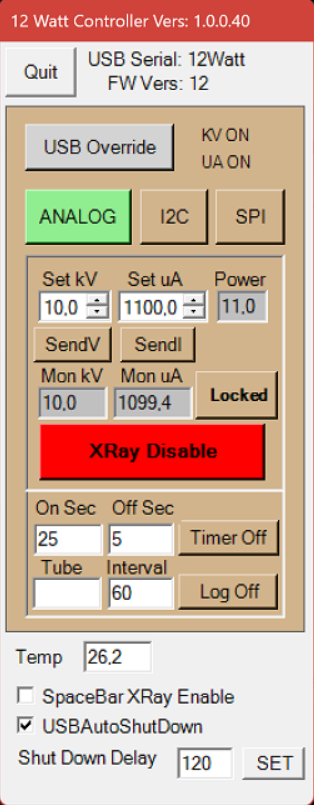
\includegraphics[width=\textwidth]{pictures/12WattController_10kV_1100uA.png}
            \caption[Set point of \qty{10}{kV} and \qty{1100}{\micro\ampere}]{Set point of \qty{10}{kV} and \qty{1100}{\micro\ampere}.}%
            \label{subfig:12WattController 10kV}
        \end{subfigure}
        \hspace{10mm}
        \begin{subfigure}{.3\textwidth}
            \centering
            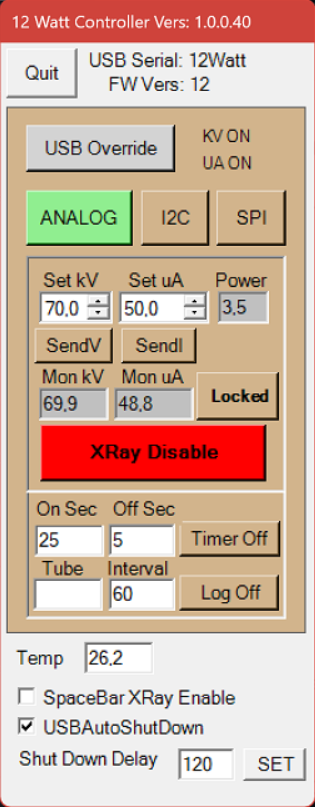
\includegraphics[width=\textwidth]{pictures/12WattController_70kV_10uA.png}
            \caption[Set point of \qty{70}{kV} and \qty{50}{\micro\ampere}]{Set point of \qty{70}{kV} and \qty{50}{\micro\ampere}.}%
            \label{subfig:12WattController 70kV}
        \end{subfigure}
        \caption[XRS GUI tool running on Windows]{XRS GUI tool running on Windows. (a) the filament current maxes out at \(\approx \qty{1100}{\micro\ampere}\). (b) a maximum acceleration voltage of \(\approx\qty{70}{\kilo\volt}\). In any case, the device does not allow exceeding a maximum power of \qty{12}{\watt}.}%
        \label{fig:12WattController 10kV and 70kV}
    \end{figure}
    \newpage
    % ===================================================================================
    \begin{figure}[t]
        \centering
        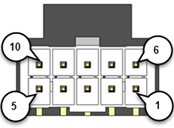
\includegraphics[width=.3\textwidth]{electronics/datasheets/XRS_10pin_male.png}
        \caption[XRS' analog control pin numbering scheme.]{XRS' analog control pin-numbering scheme.}%
        \label{fig:10 pin numbering scheme}
    \end{figure}
    \newpage
    % ===================================================================================
